\documentclass[12pt]{article}
%\usepackage[utf8]{inputenc}
%\documentclass[UTF8]{ctexart}
%\usepackage[UTF8, heading = false, scheme = plain]{ctex}
\usepackage{geometry}
%geometry{a4paper,scale=0.9}
\geometry{a4paper,left=1cm,right=1cm,top=1cm,bottom=2cm}
\usepackage{amsfonts}
\usepackage{color}
\usepackage{url}
%\usepackage{biblatex}
\usepackage{amsmath}
\usepackage{amssymb}
\usepackage{latexsym}
\usepackage{cite}
%\addbibresource{ref.bib}
%\bibliography{ref.bib}
\usepackage{caption}
\usepackage{graphicx, subfig}
\usepackage{float}
%\usepackage[fontset=ubuntu]{ctex}
%\usepackage{fontspec}
\usepackage{xeCJK}
%\usepackage[colorlinks,
%anchorcolor=black,
%citecolor=black]{hyperref}
%\setmainfont{SimSun}
\usepackage[section]{placeins}
\usepackage{enumitem}
\usepackage{framed}
\usepackage[framemethod=TikZ]{mdframed}
\usepackage{indentfirst}
\usepackage{setspace}%使用间距宏包
\linespread{1.5}
%\title{预备知识}
%\author{leolinuxer }
%\date{June 2020}

\title{关于AlphaGo\cite{Talk_About_AlphaGo}}
%\author{leolinuxer }
%\date{June 2020}

\begin{document}
\maketitle

\section{AlphaGo之前围棋 AI 的两种算法}
在 AlphaGo 之前,围棋 AI 界主要有两大类算法:Supervised Learning 和 Monte-Carlo Search:

\begin{itemize}[itemindent=2em]
    \item 监督学习 Supervised Learning(SL):直接给围棋 AI 看人类围棋大师的棋谱,让它预测人类大师的下棋位置。很显然,这就是一个分类问题:输入当前棋局状态,输出落子位置
    \item 蒙特卡洛搜索 Monte-Carlo Search:
    围棋 AI 要做的就是确定下一步棋的落子位置,换句话说,如果能评估每个下子位置的最终成功率,然后找成功率最高的就行。
\end{itemize}

对于算法来说,由于围棋的状态空间非常庞大,每一步都对应着上百个落子位置,不可能通过暴力搜索确定每个落子位置对棋局结局的贡献。这时候就得用 Monte-Carlo 法了。这个方法思路也非常简单,就是从给定落子位置开始,随机采样后续棋局(模拟),得到一个模拟的结果。经过 n 此随机采样模拟之后,将平均成功率返回作为该点的成功率。

从定性的角度上讲,Monte-Carlo 法就是用采样结果的频率来估计真实的概率。就相当于我们随机抛硬币,只要抛的次数足够多,那么,正面朝上的频率会无限接近于 0.5。这个算法的具体理论推导可以看 Sutton 的 Reinforcement Learning 那本书。

\section{AlphaGo的算法演进}
\begin{itemize}[itemindent=2em]
    \item 蒙特卡洛搜索算法,能达到 5 段左右的水平。
    
    \item 用深度卷积网络(DCNN),实现对现有棋局的监督学习,能到大约 6 段的水平。
    
    \item 在 Monte-Carlo 的采样搜索步骤中,采用前面训练好的 DCNN。因为,Monte-Carlo 法主要基于随机采样,后续的对弈对胜率的贡献其实比较小。\textbf{因此考虑在后续随机采样过程中加入人类棋手的下棋风格作为启发},就能获得更准确的估值结果。但是,DCNN 计算量太大了,一个 13 层 CNN ,计算一步落子位置就得大约 3 ms,跟 Monte-Carlo 结合效果后简直很差。
    
    \item 分类器的因为 Monte-Carlo 是纯随机采样,那么其实不需要一个太强的 DCNN,因此进一步考虑结合一个简单的分类器(Rollout policy network,简单人工提取的棋局特征 + 线性 softmax 分类器);这个分类器的特点是效果比较差,但是很快(2us)。所以和 Monte-Carlo 结合效果很好。
    
    \item 引入强化学习策略网络(RL policy network),让围棋 AI 自我对弈。基本的思路就是,让已经通过 SL 过程训练好的 AI 自我对弈,不管对弈过程,只看对弈结果。如果胜了,就给予 +1 的奖励;反之,给予 -1 的惩罚。利用返回的奖惩值指导网络权值的调整大小与方向。当然,怎么用这个 RL 策略网络依旧是一个问题。如果用它的输出结果直接进行落子判断显然效果不佳(缺乏全局观);而如果将它跟 Monte-Carlo 相结合,速度就太慢了。
    
    \item 更进一步,Monte-Carlo 就是为了估计落子位置的价值。那么,是不是可以用一个深度网络直接估计当前棋局每个位置的价值?于是,有了 AlphaGo 体系中的最后一个网络(价值网络,Value network)。这个价值网络大致结果与前面的策略网络相同(可以提取相同特征),但是最后输出的结果不再是落子位置,而是落子位置的价值(Value)。显然,这是一个回归(Regression)问题,只需在 AlphaGo 自我对弈的过程中,随机抽取棋面信息,评估该棋面状态的输赢状态,用来训练价值网络。最终,这个价值网络的估值准确率与 "Monte-Carlo + RL policy network"采样平均的估值结果接近。但是,价值网络的评估速度比它快 15000 倍。
    至此,我们便得到了 AlphaGo 所用的四种网络。
\end{itemize}

\section{AlphaGo 所用的四种网络}
\begin{figure}[ht]
  \centering
  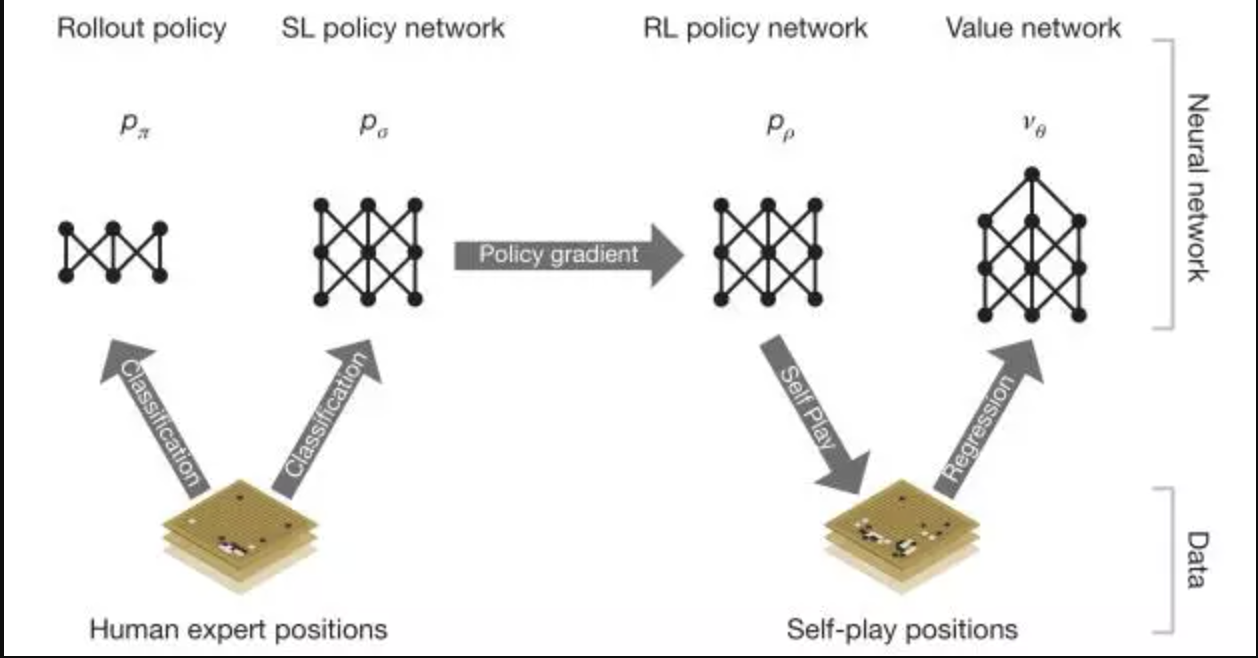
\includegraphics[width=.8\textwidth]{fig/AlphaGo的四种网络.png} %1.png是图片文件的相对路径
  \caption{AlphaGo的四种网} %caption是图片的标题
  %\label{HingeLossExample} %此处的label相当于一个图片的专属标志,目的是方便上下文的引用
\end{figure}

\begin{itemize}[itemindent=2em]
    \item Rollout Policy:快速落子网络。将很复杂的卷积神经网络去掉就能够得到一个快速走子网络。它与SL policy network的功能一样,两者间的不同是:Rollout policy网络简单,落子更快,准确率较低。
    
    \item SL Policy Network:策略网络;:用人类棋手里面的对弈记录进行训练,输入为48张图片,以输出为人类棋手的落子为目标,进行训练。
    
    \item RL Policy Network:最开始由SL policy network复制而来,两者开始对弈,在对弈的结果里面我们依据最终的胜负来修正权重。优化之后再更新对手的权重,再接着对弈,两者共同优化。
    
    \item Value Network:用RL policy network自我对弈得到的棋局数据来训练价值网络。输入是一个棋面,输出是这个棋面的胜率。为什么不直接用人类棋手的数据来训练价值网络呢?这是因为人类棋手对局的数据很少,有效样本也很少,很容易产生过拟合,对局的水平也不是很高。
\end{itemize}

在实际对弈过程中,只用了 Rollout policy network 和 Value network。也即结合价值网络和蒙特卡洛-快速走棋网络的价值评估结果。

我们最开始使用监督学习算法训练一个策略网络SL policy network,学习的资料是来自于人类棋手的对弈棋局。接下来我们训练一个RL policy network,最开始的网络结构与参数都是来自SL policy network,通过自我对弈以获得最终的胜利为目标来优化策略网络。通过这种方式就能达到一个很高的棋艺。最后,我们将训练一个价值网络 $V_{theta}$ 来预测RL policy network自我对弈的胜率。

\section{四个网络的训练方法\cite{Learning_AlphaGo}}
\subsection{Supervised learning of policy networks}
SL policy network采用卷积神经网络和ReLu激活函数,最后一层使用softmax输出落子概率。输入策略网络中的状态是一个棋盘状态的表达。如下图所示:

\begin{figure}[ht]
  \centering
  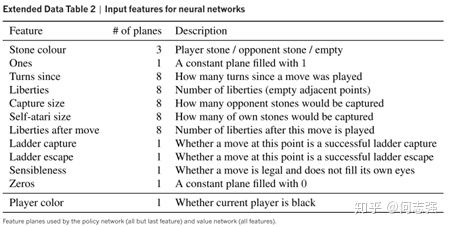
\includegraphics[width=.8\textwidth]{fig/AlphaGoSLNetworkExample.jpg} 
\end{figure}

简单来说就是48张棋局的变形,如只有黑子、只有白子、空棋盘等。用随机梯度上升去最大化其与人类棋手落子的相似度。

\subsection{Rollout Policy}
Deep Mind团队也训练一个快速走子网络Rollout Policy,Rollout Policy是一个网络结构简单的神经网络,也是使用softmax作为输出,能够达到24.2\%的精确度,决策一步棋仅需2 μs,而 SL 网络需要3 ms。这个网络主要用于后面蒙特卡洛树的模拟仿真。

\subsection{Reinforcement learning of policy networks}
RL policy network的网络结构是和SL policy network的网络结构一模一样,并且RL网络权重的初始化是拷贝SL网络的参数。使其自我博弈,随着自我博弈的进行,依据最终是否胜利RL网络就会慢慢进化。

RL policy network随机选择之前版本的自己(RL policy network)进行对弈。用这种从对手池中选择对手的方式能够更稳定地训练,防止过拟合。最终胜利的话,奖励为+1,输了的话,奖励为-1。之前也说过,这种自我对弈出来的RL policy network其实就具备很高的围棋水平了。

\subsection{Reinforcement learning of value networks}
使用RL policy network强大的策略网络来评估价值函数。价值网络的架构与策略网络的架构是非常相似的,只是将其输出变为一个单一的值,而不是策略网络中的动作分布概率。用回归的方法训练神经网络,以最小化均方差做随机梯度下降。误差来自价值网络的预测的输出和这盘局相应地最终奖励输出。为了防止过拟合等问题,他们从强化学习自我博弈的不同的棋局里面选出30万把不同位置的棋盘来做训练。

\subsection{Searching with policy and value networks}
在说这个之前我们先要说一下蒙特卡洛树搜索,这才是整个Alpha Go决策最终落字的部分,之前的深度强化学习都是为这个服务。

MCTS也就是蒙特卡罗树搜索(Monte Carlo Tree Search),是一类树搜索算法的统称,可以较为有效地解决一些探索空间巨大的问题,例如一般的围棋算法都是基于MCTS实现的。

MCTS的算法分为四步:
\begin{itemize}[itemindent=2em]
    \item 第一步是Selection,就是在树中找到一个最好的值得探索的节点,一般策略是先选择未被探索的子节点,如果都探索过就选择UCB值最大的子节点。
    
    \item 第二步是Expansion,就是在前面选中的子节点中走一步创建一个新的子节点,一般策略是随机自行一个操作并且这个操作不能与前面的子节点重复。
    
    \item 第三步是Simulation,就是在前面新Expansion出来的节点开始模拟游戏,直到到达游戏结束状态,这样可以收到到这个expansion出来的节点的得分是多少。
    
    \item 第四步是Backpropagation,就是把前面expansion出来的节点得分反馈到前面所有父节点中,更新这些节点的quality value和visit times,方便后面计算UCB值。
\end{itemize}

基本思路就是这样的,通过不断的模拟得到大部分节点的UCB值,然后下次模拟的时候根据UCB值有策略得选择值得利用和值得探索的节点继续模拟,在搜索空间巨大并且计算能力有限的情况下,这种启发式搜索能更集中地、更大概率找到一些更好的节点。

UCB: 算法本身很简单,公式如下:
$$
 \mathop{\arg\max}_{v' \in children of v} \frac{Q(v')}{N(v')} + c \sqrt{\frac{2\ln{N(v)}}{N(v'}}
$$

其中v'表示当前树节点,v表示父节点,Q表示这个树节点的累计quality值,N表示这个树节点的visit次数,C是一个常量参数(可以控制exploitation和exploration权重)。

这个公式的意思时,对每一个节点求一个值用于后面的选择,这个值有两部分组成,左边是这个节点的平均收益值(越高表示这个节点期望收益好,越值得选择,用于exploitation),右边的变量是这个父节点的总访问次数除以子节点的访问次数(如果子节点访问次数越少则值越大,越值得选择,用户exploration),因此使用这个公式是可以兼顾探索和利用的。但是在alpha go里面,将上述公式做了一定的改变。

\subsection{Monte-Carlo tree search in AlphaGo}
首先我们先有一个博弈树,博弈树是有根节点和子节点。我们把围棋的每一步所有可能选择都作为树的节点,第零层只有1个根节点,第1层就有361种下子可能和节点,第2层有360种下子可能和节点,这是一颗非常大的树,我们要在每一层树节点中搜索出赢概率最大的节点,也就是下子方法。

每条蒙特卡洛路径上面都有四个值,Q、N、P、V。Q代表这条路径的好坏,假设我们探索一条路径,最终获胜了,那么这条路径的Q值就会提升,输了的话Q值就会下降。N表示模拟走子经过这条路径的次数。最开始的Q、P都是0,P代表 $P_{\sigma}$(也就是之前说的SL policy network),是人类棋手在这条边落子的概率(之后随着网络的改进就不代表人类棋手了)。最开始的时候我们是没有子节点的,也就是与每个子节点的连接都是虚线,随着探索的增加,实边越来越多。假设我们新探索出了一条新的路径,那么这条路径的Q值与N值都将大于0,这个P一直都是$P_{\sigma}$,就是SL policy network,也就是说SL这个网络不仅是用于与强化学习对抗博弈,还用于蒙特卡洛树搜索的P值。

当我们停留在某个节点的时候,我们如何来选择动作呢?
$$
a_t = \mathop{\arg\max}_a(Q(s_t,a)+u(s_t,a))
$$
$$
u(s_t,a) \propto \frac{P(s,a)}{1+N(s,a)}
$$

我们依据上式可以知道,如果是一条没有走过的路径,那么Q值为0,但是探索度项会帮助我们提升走这条路的概率。

我们用快速走子网络进行对弈,一直下到终止,尽管快速走子网络下棋很臭,但是黑白双方都是使用快速走子网络进行对弈,从统计概念上说,他们的胜负会取决于当前棋盘的好坏,而不是网络的好坏。这个时候算出一个中间变量V:
$$
V(s_L) = (1-\lambda)v_{\theta}(s_L) + \lambda z_L
$$

再用这个中间变量V去表示Q
$$
N(s,a) = \sum_{i=1}^nl(s,a,i)
$$
$$
Q(s,a) = \frac{1}{N(s,a)}\sum_{i=1}^{n}l(s,a,i)V(s_L^i)
$$

当搜索完成之后,算法会选择最常走的那条路径进行移动。


%\printbibliography
\bibliography{../ref}
\bibliographystyle{IEEEtran}
\end{document}
